\documentclass{article}
\usepackage{graphicx} % Required for inserting images
\usepackage{subcaption}
\usepackage[T2A]{fontenc}    
\usepackage[utf8]{inputenc}  % зависит от кодировки Вашего документа
\usepackage[english,russian]{babel} 
\usepackage{float}
\usepackage{makecell}
\usepackage{mathtools}
\usepackage{blindtext}
\usepackage{titlesec}
\usepackage[clean]{svg}
\usepackage[colorlinks,urlcolor=blue]{hyperref}
\usepackage[a4paper, total={6in, 10in}]{geometry}

\title{Лабораторная работа 1}
\author{Крыжановский Максим Сергеевич}
\date{March 2024}

\begin{document}

\maketitle

\section{Постановка задачи}

В рамках задания было необходимо реализовать программу для работы с изображениями, которая включает в себя следующую функциональность:

\begin{enumerate}
    \item Загрузка изображения из файла.
    \item Сегментация изображений на основе точеченых и пространственных преобзований
    \item Бинаризацию и подсчет связных компонент, соответствующих отдельным объектам
    \item Оценка количества самолетов на фрагменте изображения
\end{enumerate}

Также было необходимо реализовать графический интерфейс для работы с программой.

\section{Программная реализация}

Программа была реализована в виде GUI-приложения на языке Python. Основным фреймворком был выбран PyQt5 для реализации графического интерфейса. Были реализованы основные морфологические операции. Всех точечных и пространственных преобразований можно достичь указав соответствующия ядра для существующих операций.

\begin{figure}[h!]
    \centering
    \includegraphics[width=0.75\linewidth]{Снимок экрана 2024-03-25 в 18.59.18.png}
    \caption{Основная страница графического интерфейса}
    \label{fig:enter-label}
\end{figure}

\section{Данные}

Перед созданием алгоритма были исследованы изображения, предлагаемые к анализу. Было обнаружено несколько важных фактов:

\begin{enumerate}
    \item Пиксели, которые относятся к самолетам имеют большую blue-составляющую в rgb представлении (зачастую больше 190)
    \item При бинаризации изображения, дорога относится к белым объектам
    \item Некоторые самолеты плохо видны на заднем плане
    \item Операции открытия и закрытия позволяют сделать самолеты более консистентными, т.е. убрать некоторые проблемы связанные с тенями на крупных самолетах
\end{enumerate}

\section{Метод решения}

Для подсчета количества самолетов был выбран следующий алгоритм:

\begin{enumerate}
    \item Операции открытия и закрытия для удаления шумовых точек
    \item Бинаризация изображения в соответствии с цветовой палитрой
    \item Определение связных компонент
    \item Обведение связных компонент на изображении
\end{enumerate}

\subsection{Предобработка перед бинаризацией}

Перед бинаризацией по цвету было решено провести ряд морфологических операций:

\begin{enumerate}
    \item Открытие с ядро размера 4x4 из единиц
    \item Закрытие с ядром размера 3x3 из единиц
\end{enumerate}

Предполагается, что данные преобразования помогут бороться с шумовыми точками и лучше объединить связные компоненты самолетов.

\begin{figure}[h!]
    \centering
    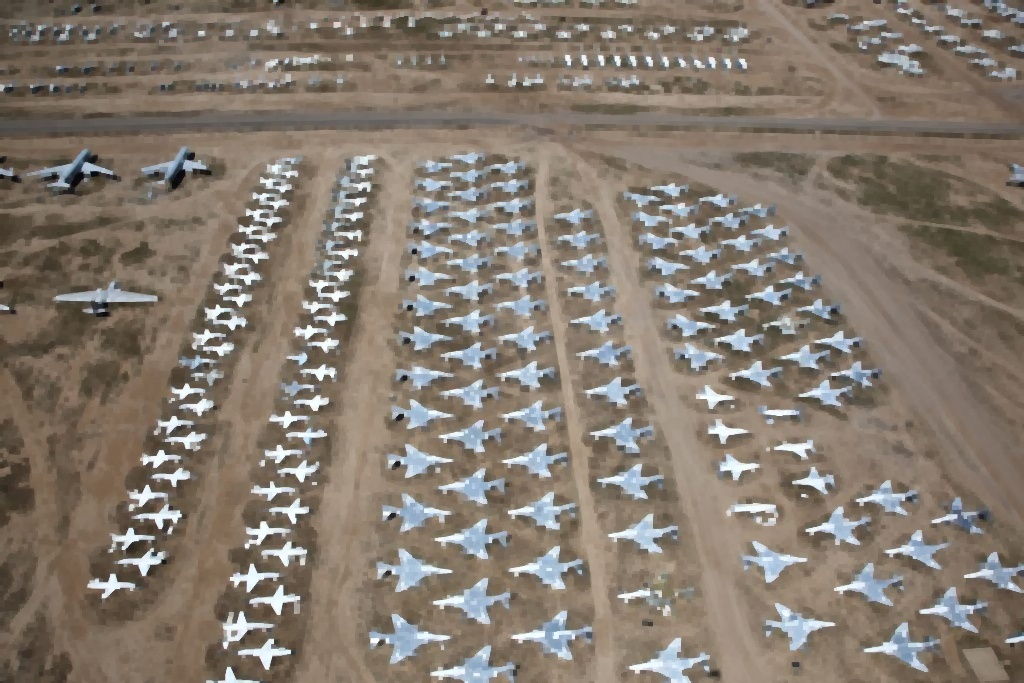
\includegraphics[width=0.5\linewidth]{1_new.jpg}
    \caption{Изображение после проведения операций закрытия и открытия}
    \label{fig:enter-label}
\end{figure}

\subsection{Бинаризация изображения}

Бинаризация изображения производилась на основе отбора по цветовой гамме. Были изучены rgb-значения пикселей на изображениях. Бали установлены следующие пороги:

\begin{enumerate}
    \item Все пиксели с компонентой blue со значением выше 195 - белые
    \item Все оставшиеся пиксели - черные
\end{enumerate}

\begin{figure}[h!]
  \centering
  \begin{subfigure}[b]{0.4\linewidth}
    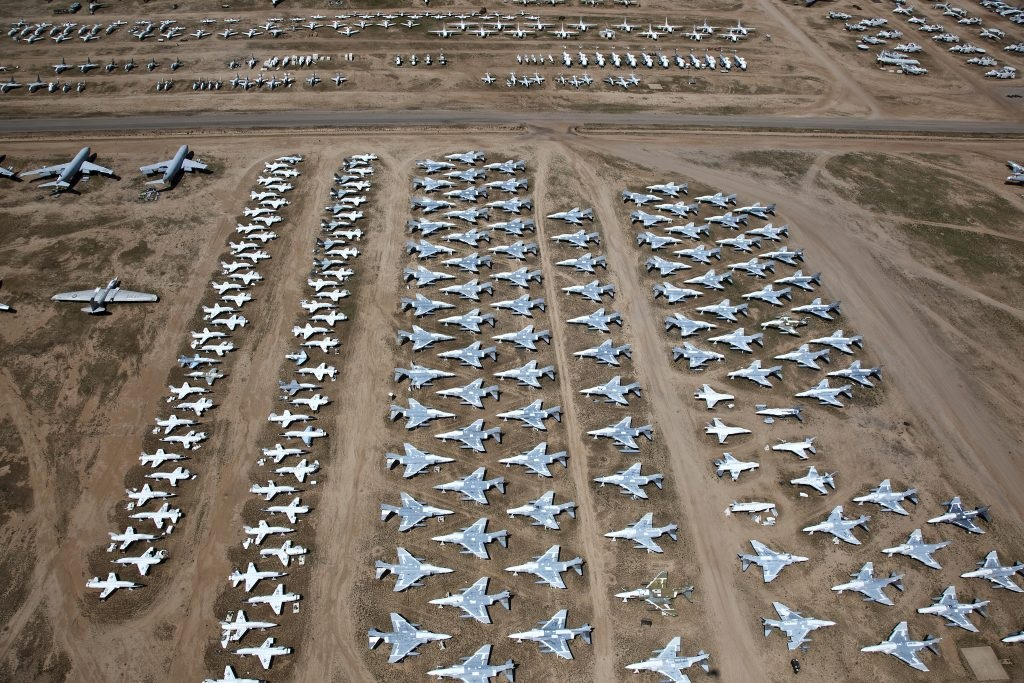
\includegraphics[width=\linewidth]{1.jpg}
    \caption{Фото до бинаризации}
    \label{fig:sub1}
  \end{subfigure}
  \begin{subfigure}[b]{0.4\linewidth}
    \includegraphics[width=\linewidth]{blcak-white.png}
    \caption{Фото после бинаризации}
    \label{fig:sub2}
  \end{subfigure}
  \caption{Пример работа алгоритма бинаризации}
  \label{fig:twophotos}
\end{figure}

\subsection{Определение связных компонент}

Связные компоненты определялись как соседние пиксели белого цвета. Пиксели считаются соседними, если они связаны по вертикали или по горизонтали, но не по диагонали. Данный алгоритм был реализован с помощью инструментов биьблиотеки cv2 и функции findCountours.

\begin{figure}[h!]
  \centering
  \begin{subfigure}[b]{0.4\linewidth}
    \includegraphics[width=\linewidth]{blcak-white.png}
    \caption{Бинарная фотография}
    \label{fig:sub1}
  \end{subfigure}
  \begin{subfigure}[b]{0.4\linewidth}
    \includegraphics[width=\linewidth]{highlighted.png}
    \caption{После выделения компонент}
    \label{fig:sub2}
  \end{subfigure}
  \caption{Пример выделения связаных компонент}
  \label{fig:twophotos}
\end{figure}

\subsection{Подсчет связных компонент и обведение компонентов}

При подсчете связных компоненты мы не учитывали компоненты, площадь которых была меньше или равна 20 пикселям. Выделение связных компонент было проведено с использованием средств библиотеки cv2 и функции drawCountours.

\section{Иллюстрация работы программы}

В данном разделе продемострируем некоторые примеры работы приложения, которое было реализовано в рамках задания.

\begin{figure}[h!]
    \centering
    \includegraphics[width=0.5\linewidth]{Снимок экрана 2024-03-25 в 22.04.11.png}
    \caption{Подсчет и выделение самолетов в приложении}
    \label{fig:enter-label}
\end{figure}

\begin{figure}[h!]
    \centering
    \includegraphics[width=0.5\linewidth]{Снимок экрана 2024-03-25 в 22.04.25.png}
    \caption{Применение эрозии в приложении}
    \label{fig:enter-label}
\end{figure}

Также в приложении при использовании преобразований можно устанавливать собственные ядра. По умолчанию во всех операциях используется ядро размера 5x5, состоящее из единиц. Для установки ядра необходмо в строку через пробел ввести все элементы матрицы ядра. Элементы будут построчно перенесны в матрицу в соответствии с C-порядком.

\begin{figure}[h!]
    \centering
    \includegraphics[width=0.5\linewidth]{Снимок экрана 2024-03-25 в 22.07.36.png}
    \caption{Пример установки пользовательского ядра}
    \label{fig:enter-label}
\end{figure}

Также реализована функция бинаризации и пользовательского фильтра.

\begin{figure}[h!]
    \centering
    \includegraphics[width=0.5\linewidth]{Снимок экрана 2024-03-25 в 22.17.10.png}
    \caption{Пример бинаризации}
    \label{fig:enter-label}
\end{figure}

\end{document}